\documentclass[10pt]{beamer}

\usetheme{Madrid}
\usecolortheme{default}
\setbeamertemplate{navigation symbols}{}
\setbeamersize{text margin left=0.6cm,text margin right=0.6cm}

\usepackage{tikz}
\usetikzlibrary{shapes, arrows.meta, positioning, fit, calc}
\usepackage{amsmath, amssymb}
\pdfstringdefDisableCommands{\def\translate#1{#1}}

\title[Introduction to ToC]{Introduction to the Theory of Computation}
\subtitle{Mathematical Foundations and Preliminaries}
\author[SDB]{}
\date[Slide Set 1]{\scriptsize \textit{Theory of Computation Slide Sets}}

\begin{document}

\begin{frame}
  \titlepage
\end{frame}

\begin{frame}{Table of Contents}
  \tableofcontents
\end{frame}

\begin{frame}{Learning Outcomes and Notation}
  \small
  By the end of this set, you should be able to:
  \begin{itemize}
    \item use sets, functions, relations, and quantifiers precisely;
    \item distinguish walks, cycles, rooted trees, depth, and height;
    \item manipulate strings and languages, including their empty cases;
    \item distinguish a problem, an instance, a solution, and an algorithm,
      and encode a finite instance as a string;
    \item distinguish generating a language from recognizing or deciding it;
    \item view computation as a string-to-string transformation and explain
      why different models help us study it;
    \item choose and write a direct, contrapositive, contradiction, or
      induction proof.
  \end{itemize}
  \pause
  \begin{block}{Conventions used throughout these slide sets}
    $\mathbb{N}=\{0,1,2,\ldots\}$; $\mathbb{Z}$ denotes the integers.
    $|S|$ is a set's cardinality, whereas $|w|$ is a string's length.
    An alphabet is finite and nonempty. A word means a finite string.
    Unless stated otherwise, graphs and trees here are finite.
  \end{block}
  Definitions and proof patterns are the prerequisites; the appendix
  supplies worked answers and further examples for independent practice.
\end{frame}

% ==========================================
% Part 1: Overview of Computation
% ==========================================
\section{Overview of Computation}

\begin{frame}{Part 1: The Big Question}
  \small
  \begin{block}{The Fundamental Question}
    \textbf{What are the fundamental capabilities and limitations of computers?}
  \end{block}
  \pause
  \vspace{0.5cm}
  To answer this rigorously, theoretical computer science rests on three pillars:
  \pause
  \begin{itemize}
      \item \textbf{Automata Theory:} How do we model computation? Finite
        automata, pushdown automata, and Turing machines provide precise
        models with different memory capabilities.
      \pause
      \item \textbf{Computability Theory:} What is solvable vs. unsolvable? We determine if an algorithm can exist for a given problem (e.g., the Halting Problem).
      \pause
      \item \textbf{Complexity Theory:} What is computationally easy vs. hard? We classify problems based on resource requirements like time and space (e.g., P vs. NP).
  \end{itemize}
\end{frame}

% ==========================================
% Part 2: Sets, Sequences, and Tuples
% ==========================================
\section{Sets, Sequences, and Tuples}

\begin{frame}{Part 2: Sets and Basics}
  \small
  A \textbf{set} is a collection of distinct objects, called its
  \textbf{elements}. Order and repeated listings do not matter:
  $\{a,b,a\}=\{b,a\}$.
  \pause
  \begin{itemize}
      \item \textbf{Membership:} $x \in S$ means $x$ is an element of $S$. $x \notin S$ means it is not.
      \item \textbf{Subset:} $A \subseteq B$ means every element of $A$ is also in $B$.
      \item \textbf{Empty Set:} $\emptyset$ is the set with no elements.
      \item \textbf{Set-builder notation:}
        $\{n\in\mathbb{N}:n\text{ is even}\}=\{0,2,4,\ldots\}$.
  \end{itemize}
  \pause
  
  \begin{alertblock}{Membership is not containment}
    For $S=\{a,b\}$, $a\in S$, but $\{a\}\subseteq S$.
    Also $\emptyset\subseteq S$, while $\emptyset\notin S$.
    The set $\{\emptyset\}$ has one element, so it is not empty.
    \par\smallskip
    To prove $A=B$, prove both $A\subseteq B$ and $B\subseteq A$.
  \end{alertblock}
\end{frame}

\begin{frame}{Set Operations and Venn Diagrams}
  \small
  Let $A,B\subseteq U$, where $U$ is the fixed universe.
  \begin{columns}[T]
    \column{0.46\textwidth}
    \begin{itemize}
        \item \textbf{Union} ($A \cup B$): Elements in $A$ or $B$ or both.
        \item \textbf{Intersection} ($A \cap B$): Elements in both.
        \item \textbf{Difference} ($A - B$ or $A \setminus B$): Elements in $A$ but not $B$.
        \item \textbf{Complement}: $\overline{A}=U\setminus A$.
    \end{itemize}
    
    \column{0.52\textwidth}
    \begin{center}
    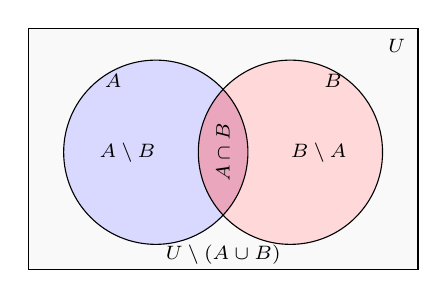
\begin{tikzpicture}[scale=0.9,every node/.style={font=\scriptsize}]
      \draw[fill=gray!5] (-1.8,-1.65) rectangle (3.7,1.75);
      \fill[blue!15] (0,0) circle (1.3);
      \fill[red!15] (1.9,0) circle (1.3);
      \begin{scope}
        \clip (0,0) circle (1.3);
        \fill[purple!35] (1.9,0) circle (1.3);
      \end{scope}
      \draw (0,0) circle (1.3);
      \draw (1.9,0) circle (1.3);
      \node at (-0.4,0) {$A\setminus B$};
      \node at (2.3,0) {$B\setminus A$};
      \node[rotate=90] at (0.95,0) {$A\cap B$};
      \node at (-0.6,1) {$A$};
      \node at (2.5,1) {$B$};
      \node at (3.4,1.5) {$U$};
      \node at (0.95,-1.45) {$U\setminus(A\cup B)$};
    \end{tikzpicture}
    \end{center}
  \end{columns}
  \pause
  \begin{block}{De Morgan's laws: negate the membership condition}
    $\overline{A\cup B}=\overline{A}\cap\overline{B}$,
    \qquad $\overline{A\cap B}=\overline{A}\cup\overline{B}$.
    \par\smallskip
    All complements must use the same universe.
  \end{block}
\end{frame}

\begin{frame}{Power Sets and Cartesian Products}
  \small
  \begin{block}{Power Set}
    The \textbf{power set} of $S$, denoted $2^S$ (or $\mathcal{P}(S)$), is the set of all subsets of $S$.
    \newline \textbf{Example:} If $S = \{a, b, c\}$, then:
    $$2^S = \{\emptyset, \{a\}, \{b\}, \{c\}, \{a, b\}, \{a, c\}, \{b, c\}, \{a, b, c\}\}$$
    For finite $S$, $|2^S|=2^{|S|}$: independently include or exclude each
    element. In particular, $2^{\emptyset}=\{\emptyset\}$ has size $1$.
  \end{block}
  \pause
  \begin{block}{Sequences, Tuples, and Cartesian Products}
    A \textbf{sequence} is an ordered list; repetitions are allowed.
    A finite sequence is a \textbf{tuple}; $(a,b)=(c,d)$ iff $a=c$ and $b=d$.
    \newline \textbf{Cartesian Product} ($A \times B$): The set of all ordered pairs $(a, b)$ where $a \in A$ and $b \in B$.
    \newline \textbf{Example:} $A = \{1, 2\}$, $B = \{x, y, z\}$
    $$A \times B = \{(1, x), (1, y), (1, z), (2, x), (2, y), (2, z)\}$$
    For finite sets, $|A\times B|=|A||B|$. If either factor is empty,
    the product is empty.
  \end{block}
\end{frame}

% ==========================================
% Part 3: Functions and Relations
% ==========================================
\section{Functions, Relations, and Logic}

\begin{frame}{Part 3: Functions}
  \small
  A \textbf{function} (or mapping) $f : D \rightarrow C$ assigns exactly one element in the \textbf{codomain} $C$ to each element in the \textbf{domain} $D$.
  \pause
  \begin{itemize}
      \item \textbf{Range:} The subset of the codomain containing all actual outputs, defined as $f(D) = \{f(x) \mid x \in D\} \subseteq C$.
      \pause
      \item \textbf{Total Function:} Defined for \textit{every} element in the domain $D$.
      \pause
      \item \textbf{Partial Function:} $f:D\rightharpoonup C$ assigns an
        output to each element of some subset of $D$; other inputs have
        no defined output. Ordinary $f:D\to C$ means a total function here.
  \end{itemize}
  \pause
  \vspace{0.2cm}
  \begin{exampleblock}{Example}
    For $f:\mathbb{Z}\to\mathbb{Z}$, $f(x)=|x|$, the range is
    $\mathbb{N}=\{0,1,2,\ldots\}$, not all of the codomain $\mathbb{Z}$.
  \end{exampleblock}
  \textbf{Bridge to deterministic finite automata (DFAs):} their transition
  function is total. A missing arrow must be handled explicitly, usually
  by a rejecting sink state. A nondeterministic finite automaton (NFA)
  can instead return the empty \emph{set} of successor states.
\end{frame}

\begin{frame}{Part 3: Properties of Functions}
  \small
  Functions are classified by how elements in the domain map to the codomain:
  \pause
  \begin{itemize}
      \item \textbf{Injective (One-to-One):} Distinct inputs always map to distinct outputs. If $f(a) = f(b)$, then $a = b$. No two arrows point to the same target.
      \pause
      \item \textbf{Surjective (Onto):} Every element in the codomain is mapped to by at least one element in the domain. The \textbf{range equals the codomain}.
      \pause
      \item \textbf{Bijective (One-to-One Correspondence):} Both injective and surjective. Every input has a unique output, and every output has a unique input. Essential for defining \textbf{inverse functions}.
  \end{itemize}
  \pause
  % \vspace{-0.2cm}
  \begin{exampleblock}{Quick Check}
    \begin{itemize}
        \item $f: \mathbb{R} \rightarrow \mathbb{R}, f(x) = x^3$ is \textbf{bijective}.
        \item $f:\mathbb{R}\to\mathbb{R}$, $f(x)=x^2$ is \textbf{neither}:
          $f(-1)=f(1)$, and no input maps to $-1$.
    \end{itemize}
  \end{exampleblock}
  Changing domain and codomain matters: $x\mapsto x^2$ from
  $[0,\infty)$ to $[0,\infty)$ is bijective, with inverse $x\mapsto\sqrt{x}$.
  For $f:D\to C$ and $g:C\to E$, composition is read right to left:
  $(g\circ f)(x)=g(f(x))$.
\end{frame}


\begin{frame}{Relations and Equivalence}
  \small
  A $k$-ary \textbf{relation} is a subset of a Cartesian product of $k$ sets.
  A binary relation $R$ on $A$ is a subset of $A\times A$.
  Write $aRb$ for $(a,b)\in R$. A relation need not be a function.
  \pause
  \begin{block}{Equivalence Relation}
    A binary relation $R$ is an \textbf{equivalence relation} if it satisfies three conditions:
    \begin{enumerate}
        \item \textbf{Reflexivity:} $xRx$ for every $x$.
        \item \textbf{Symmetry:} If $xRy$, then $yRx$.
        \item \textbf{Transitivity:} If $xRy$ and $yRz$, then $xRz$.
    \end{enumerate}
  \end{block}
  \pause
  \begin{alertblock}{Equivalence Classes}
    Define $[a]_R=\{b\in A:aRb\}$. These classes cover $A$; any two
    are equal or disjoint. Thus the distinct classes form a partition.
    State minimization later groups states with the same future behavior.
  \end{alertblock}
\end{frame}

\begin{frame}{Worked Equivalence Relation: Remainders Modulo Three}
  \small
  On $\mathbb{Z}$, define $x\sim y$ iff $3$ divides $x-y$.
  Equivalently, $x$ and $y$ have the same remainder modulo $3$.
  \begin{itemize}
    \item \textbf{Reflexive:} $x-x=0$ is divisible by $3$.
    \item \textbf{Symmetric:} if $x-y=3k$, then $y-x=3(-k)$.
    \item \textbf{Transitive:} if $x-y=3k$ and $y-z=3\ell$,
      then $x-z=3(k+\ell)$.
  \end{itemize}
  \pause
  There are exactly three classes:
  \[
    \begin{aligned}
      {}[0]&=\{\ldots,-6,-3,0,3,6,\ldots\},\\
      [1]&=\{\ldots,-5,-2,1,4,7,\ldots\},\\
      [2]&=\{\ldots,-4,-1,2,5,8,\ldots\}.
    \end{aligned}
  \]
  \pause
  For example, $[4]=[1]$, not a fourth class. A machine checking a count
  modulo three can remember its class instead of the entire count.
\end{frame}

\begin{frame}{Boolean Logic}
  \small
  Boolean logic uses values TRUE ($1$) and FALSE ($0$). We build complex expressions using boolean operations:
  \pause
  \begin{itemize}
      \item \textbf{NOT ($\neg$):} $\neg 0 = 1$ and $\neg 1 = 0$.
      \item \textbf{AND ($\wedge$):} $1 \wedge 1 = 1$, all other combinations are $0$.
      \item \textbf{OR ($\vee$):} $0 \vee 0 = 0$, all other combinations are $1$.
  \end{itemize}
  \pause
  \begin{block}{Precedence}
    Just like arithmetic ($\times$ before $+$), boolean operations have an evaluation order: 
    \begin{center}
      \textbf{NOT precedes AND, and AND precedes OR.}
    \end{center}
    Example: $P \vee Q \wedge \neg R$ is evaluated as $P \vee (Q \wedge (\neg R))$.
  \end{block}
\end{frame}

\begin{frame}{Implication, Equivalence, and Counterexamples}
  \small
  \begin{block}{Implication is not a claim of causation}
    $P\Rightarrow Q$ means ``if $P$, then $Q$'' and is equivalent to
    $\neg P\vee Q$. It is false only when $P$ is true and $Q$ is false.
    $P\Leftrightarrow Q$ requires both $P\Rightarrow Q$ and $Q\Rightarrow P$.
  \end{block}
  \pause
  \begin{itemize}
    \item The \textbf{contrapositive} $\neg Q\Rightarrow\neg P$ is equivalent
      to $P\Rightarrow Q$.
    \item The \textbf{converse} $Q\Rightarrow P$ need not follow.
      Divisibility by $4$ implies evenness, but $6$ refutes the converse.
    \item To refute a universal implication, find one case where the
      hypothesis holds and the conclusion fails. Positive examples alone
      do not prove a universal claim.
  \end{itemize}
  \pause
  \textbf{Vacuous truth:} if no object satisfies the hypothesis, there is
  no counterexample. This is why $\emptyset\subseteq A$ for every set $A$.
\end{frame}

\begin{frame}{Quantifiers: Who May Depend on Whom?}
  \small
  $\forall x\in D$ means ``for every $x$ in $D$'';
  $\exists x\in D$ means ``for at least one $x$ in $D$.''
  Always state the domain.
  \begin{exampleblock}{Changing the order changes the claim}
    $\forall n\in\mathbb{N}\;\exists m\in\mathbb{N}:m>n$ is true;
    choose $m=n+1$, depending on $n$.
    \par\smallskip
    $\exists m\in\mathbb{N}\;\forall n\in\mathbb{N}:m>n$ is false;
    the proposed fixed $m$ fails when $n=m$.
  \end{exampleblock}
  \pause
  \begin{block}{Negation swaps the quantifier and negates its body}
    \[
      \neg(\forall x\in D\;P(x))\iff\exists x\in D\;\neg P(x),
    \]
    \[
      \neg(\exists x\in D\;P(x))\iff\forall x\in D\;\neg P(x).
    \]
  \end{block}
  Over an empty domain, a universal statement is true and an existential
  statement is false. Quantifier order will be central to pumping arguments.
\end{frame}

% ==========================================
% Part 4: Graphs and Trees
% ==========================================
\section{Graphs and Trees}

\begin{frame}{Part 4: Graph Theory Basics}
  \small
  A \textbf{graph} $G = (V, E)$ consists of a set of vertices (nodes) $V$ and a set of edges $E$.
  \vspace{5mm}
  \pause
  \begin{columns}
    \column{0.5\textwidth}
    \textbf{Simple undirected graph:} $E$ contains unordered pairs
    $\{u,v\}$ with $u\ne v$; no loops or parallel edges.
    \begin{center}
    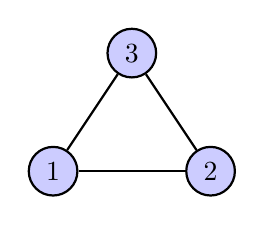
\begin{tikzpicture}[scale=1, auto, thick]
      \node[draw, circle, fill=blue!20] (1) at (0, 0) {1};
      \node[draw, circle, fill=blue!20] (2) at (2, 0) {2};
      \node[draw, circle, fill=blue!20] (3) at (1, 1.5) {3};
      \draw (1) -- (2);
      \draw (2) -- (3);
      \draw (3) -- (1);
    \end{tikzpicture}
    \end{center}
    
    \column{0.5\textwidth}
    \textbf{Directed Graph (Digraph):} Edges have direction. $E$ consists of ordered pairs $(u, v)$.
    \begin{center}
    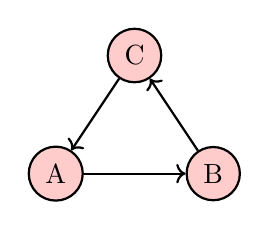
\begin{tikzpicture}[scale=1, auto, thick]
      \node[draw, circle, fill=red!20] (A) at (0, 0) {A};
      \node[draw, circle, fill=red!20] (B) at (2, 0) {B};
      \node[draw, circle, fill=red!20] (C) at (1, 1.5) {C};
      \draw[->] (A) -- (B);
      \draw[->] (B) -- (C);
      \draw[->] (C) -- (A);
    \end{tikzpicture}
    \end{center}
  \end{columns}
  \vspace{0.2cm}
  A \textbf{walk} follows adjacent edges (respecting direction in a digraph);
  its length is its number of edges. A \textbf{simple path} repeats no vertex.
  A \textbf{cycle} is a nonempty closed walk with no repeated edge and no
  repeated vertex other than its initial/final vertex. Automata diagrams may have loops and labels;
  their computations are walks, often called paths in automata texts.
\end{frame}

\begin{frame}{Tree Structures}
  \small
  An undirected \textbf{tree} is a connected graph with no cycles.
  Choose a \textbf{root} and orient each edge away from it: the root has
  no parent, every other node has exactly one parent, and nodes with no
  children are \textbf{leaves}. A single root is also a tree and a leaf.
  
  \begin{center}
  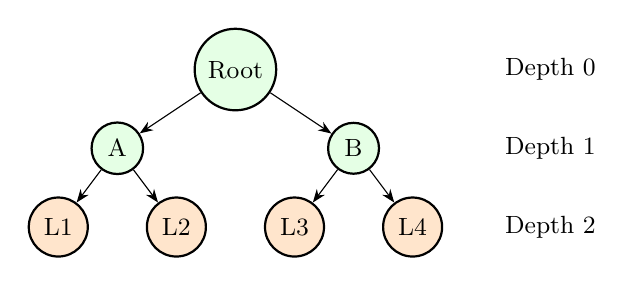
\begin{tikzpicture}[level distance=1cm,>=Stealth,edge from parent/.style={draw,->},
    level 1/.style={sibling distance=3cm},
    level 2/.style={sibling distance=1.5cm},
    every node/.style={draw, circle, fill=green!10, thick,font=\small}]
    
    \node (Root) {Root}
      child {node {A}
        child {node[fill=orange!20] {L1}}
        child {node[fill=orange!20] {L2}}
      }
      child {node {B}
        child {node[fill=orange!20] {L3}}
        child {node[fill=orange!20] {L4}}
      };
      
    \node[draw=none,fill=none,rectangle] at (4,0) {Depth 0};
    \node[draw=none,fill=none,rectangle] at (4,-1) {Depth 1};
    \node[draw=none,fill=none,rectangle] at (4,-2) {Depth 2};
  \end{tikzpicture}
  \end{center}
  \pause
  \textbf{Depth} is the number of edges from the root to a node.
  \textbf{Height} of a node is the longest downward path to a leaf;
  the tree's height is its root's height (here $2$).
  A \textbf{binary tree} has at most two children per node.
  In an \textbf{ordered tree}, the left-to-right child order matters.
\end{frame}

% ==========================================
% Part 5: Strings and Languages
% ==========================================
\section{Strings and Languages}

\begin{frame}{Part 5: Alphabets and Strings}{Fundamental Data Types of Computation}
  \small
  \begin{itemize}
      \item \textbf{Alphabet ($\Sigma$):} A finite, nonempty set of symbols. \\Example: $\Sigma = \{0, 1\}$ or $\Sigma = \{a, b, \dots, z\}$.
      \pause
      \item \textbf{String:} A finite sequence of symbols from $\Sigma$.
      \item \textbf{Length ($|w|$):} The number of symbols in string $w$. If $w = 1011$, $|w| = 4$.
      \pause
      \item \textbf{Empty String ($\varepsilon$ or $\lambda$):} The string of length zero. $|\varepsilon| = 0$.
      \item \textbf{Concatenation:} Appending strings. If $x = 01$ and $y = 11$, $xy = 0111$.
      \item \textbf{Reversal ($w^R$):} The string written backwards. $(011)^R = 110$.
  \end{itemize}
  The symbol $\varepsilon$ denotes a word with no symbols; it is not an
  extra input symbol in $\Sigma$.
\end{frame}

\begin{frame}{String Operations and Positions}
  \small
  Concatenation is associative: $(xy)z=x(yz)$, with identity
  $x\varepsilon=\varepsilon x=x$. It is not generally commutative:
  $01\ne10$.
  \[
    |xy|=|x|+|y|,\qquad (xy)^R=y^Rx^R,\qquad (w^R)^R=w.
  \]
  Define $w^0=\varepsilon$ and $w^{n+1}=w^n w$; thus $(01)^3=010101$.
  \pause
  \begin{block}{Prefix, suffix, substring, subsequence}
    $u$ is a \textbf{prefix} of $w$ if $w=uv$ for some $v$; a
    \textbf{suffix} if $w=vu$; a \textbf{substring} if $w=xuy$.
    A \textbf{subsequence} is obtained by deleting zero or more symbols,
    without changing the order of those retained.
    \par\smallskip
    In $w=0101$, $010$ is a prefix, $101$ a suffix, and $10$ a substring.
    The word $00$ is a subsequence but not a substring.
  \end{block}
  \pause
  The empty word is a prefix, suffix, substring, and subsequence of every
  word. A substring must be contiguous; a subsequence need not be.
\end{frame}

\begin{frame}{Languages and the Kleene Star}
  \small
  \begin{block}{Kleene Star ($\Sigma^*$)}
    Let $\Sigma^n$ be the set of strings of length $n$, with
    $\Sigma^0=\{\varepsilon\}$. Then
    $\Sigma^*=\bigcup_{n\ge0}\Sigma^n$ and
    $\Sigma^+=\bigcup_{n\ge1}\Sigma^n=\Sigma^*\setminus\{\varepsilon\}$.
    \newline Example: If $\Sigma = \{0, 1\}$, then $\Sigma^* = \{\varepsilon, 0, 1, 00, 01, 10, 11, 000, \dots\}$.
  \end{block}
  \pause
  % \vspace{-2mm}
  \begin{block}{Formal Language}
    A \textbf{language} $L$ is simply a subset of $\Sigma^*$. 
    $$L \subseteq \Sigma^*$$
    A language can be finite or infinite. Even the empty set $\emptyset$ is a language.
  \end{block}
  \pause
  \begin{alertblock}{Keep the empty cases separate}
    $\emptyset$ is a language with zero words; $\{\varepsilon\}$ is a language
    with one word; $\varepsilon$ is a word of length zero.
    Thus $|\emptyset|=0$, $|\{\varepsilon\}|=1$, and $|\varepsilon|=0$.
    A language is a set: listing a word twice does not create another element.
  \end{alertblock}
\end{frame}

\begin{frame}{Operations on Languages}
  \small
  For $L,K\subseteq\Sigma^*$, union and intersection are ordinary set
  operations; complement means $\Sigma^*\setminus L$ for the fixed alphabet.
  \begin{block}{Concatenation and repetition}
    \[
      LK=\{xy:x\in L,\ y\in K\},\qquad L^R=\{w^R:w\in L\},
    \]
    \[
      L^0=\{\varepsilon\},\quad L^{n+1}=L^nL,\quad
      L^*=\bigcup_{n\ge0}L^n,\quad L^+=\bigcup_{n\ge1}L^n.
    \]
    Each factor may be a \emph{different} word of $L$.
  \end{block}
  \pause
  For $L=\{a,bb\}$, $L^2=\{aa,abb,bba,bbbb\}$.
  \[
    L\{\varepsilon\}=\{\varepsilon\}L=L,\qquad L\emptyset=\emptyset L=\emptyset,
    \qquad \emptyset^*=\{\varepsilon\}.
  \]
  \pause
  \begin{alertblock}{A plus does not always exclude the empty word}
    $L^+$ means one or more \emph{factors}. If $\varepsilon\in L$, then
    $\varepsilon\in L^+$ too. The identity $L^+=L^*\setminus\{\varepsilon\}$
    holds when $\varepsilon\notin L$, as for an alphabet's one-symbol words.
  \end{alertblock}
\end{frame}

\begin{frame}{Counting Words and the Pigeonhole Principle}
  \small
  If $|\Sigma|=k$, then $|\Sigma^n|=k^n$: each of the $n$ positions has
  $k$ independent choices. For $n=0$, there is one word, not zero words.
  \begin{exampleblock}{Binary words}
    Length three: $000,001,010,011,100,101,110,111$.
    Length at most three: $1+2+4+8=15$ words, including $\varepsilon$.
  \end{exampleblock}
  \pause
  \begin{block}{Pigeonhole principle}
    Placing more than $r$ objects into $r$ boxes forces some box to contain
    at least two objects. Otherwise the total could not exceed $r$.
  \end{block}
  \pause
  A run that visits $r+1$ states in a machine with only $r$ states repeats
  a state. A DFA reading $r$ symbols has $r+1$ visits, counting its start.
  This does not itself imply acceptance; it identifies repeated behavior
  that later proofs can exploit.
\end{frame}

\begin{frame}{Problems, Instances, Solutions, and Algorithms}
  \small
  A \textbf{computational problem} specifies allowed inputs and the outputs
  considered correct. An \textbf{instance} is one particular input.
  A \textbf{solution to an instance} is a correct output, not the procedure
  used to obtain it.
  \begin{exampleblock}{Sorting as a running example}
    \textbf{Problem:} given a finite list of integers, return the same
    elements, with the same multiplicities, in nondecreasing order.
    \par\smallskip
    \textbf{Instance:} $(3,1,3,2)$.
    \quad\textbf{Solution:} $(1,2,3,3)$.
    Removing a repeated $3$ would give an incorrect solution.
  \end{exampleblock}
  \pause
  \begin{block}{A specification is not an algorithm}
    With one specified answer per input, the problem is a function
    $f:I\to O$: it states \emph{what} output belongs to each input.
    An \textbf{algorithm computing $f$} is a finite, effective procedure
    that halts with output $f(x)$ for every permitted input $x$.
    It states \emph{how} to obtain the answer.
  \end{block}
  Some tasks allow several outputs (for example, any valid route).
  Specify the allowed answers, or fix a selection rule to obtain a function.
  Defining an input--output requirement does not guarantee an algorithm
  exists~\cite{algorithms-intro}.
\end{frame}

\begin{frame}{What Does Encoding an Instance as a String Mean?}
  \small
  An \textbf{encoding} is an agreed representation of structured data by
  symbols from a finite alphabet. Writing $\langle x\rangle$ means
  ``the chosen string representation of the instance $x$.''
  \begin{block}{What the format must specify}
    \begin{itemize}
      \item How numbers, vertices, lists, and other components are written.
      \item How component boundaries and their order can be recovered.
      \item Which strings are well-formed and how to decode them.
    \end{itemize}
    We choose an effective, unambiguous format. A canonical encoding
    $\operatorname{enc}:I\to\Sigma^*$ is injective and satisfies
    $\operatorname{decode}(\operatorname{enc}(x))=x$.
  \end{block}
  \pause
  \textbf{Example:} the number $13$ can be represented in binary as
  \texttt{1101}. The number is the object; the four-symbol word is its encoding.
  Encoding need not be encryption or compression.
  \pause
  \par\smallskip
  The \textbf{input length} is $m=|\langle x\rangle|$, not necessarily the
  numerical value of $x$ or the number of objects in it. Algorithms read
  representations; a decoder connects those strings to their meaning.
\end{frame}

\begin{frame}{Worked Encoding: A Graph and a Reachability Question}
  \small
  An instance is $(G,s,t)$: a labeled directed graph and two designated
  vertices. Does a directed path lead from $s$ to $t$?
  \begin{columns}[T]
    \column{0.46\textwidth}
    \centering
    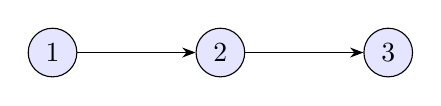
\begin{tikzpicture}[>=Stealth,node distance=1.5cm,
        vertex/.style={draw,circle,fill=blue!10}]
      \node[vertex] (one) {$1$};
      \node[vertex,right=of one] (two) {$2$};
      \node[vertex,right=of two] (three) {$3$};
      \draw[->] (one) -- (two);
      \draw[->] (two) -- (three);
    \end{tikzpicture}
    \par\smallskip $n=3,\ s=1,\ t=3$
    \column{0.50\textwidth}
    $A_{ij}=1$ iff $i\to j$ is an edge:
    \[
      A=\begin{pmatrix}0&1&0\\0&0&1\\0&0&0\end{pmatrix}.
    \]
  \end{columns}
  \pause
  Use alphabet $\{0,1,\#\}$ and the format
  \[
    \langle G,s,t\rangle=\text{bin}(n)\#
      \text{rows}(A)\#\text{bin}(s)\#\text{bin}(t).
  \]
  Here vertices are $1,\ldots,n$; positive integers use binary without
  leading zeros; $\text{rows}(A)$ lists exactly $n^2$ bits row by row.
  \[
    \boxed{\texttt{11\#010001000\#1\#11}}
  \]
  \pause
  Decoding recovers the graph and endpoints, not the answer. The answer
  is \texttt{YES}, with path $(1,2,3)$. A valid encoding with endpoints
  reversed is a \emph{no-instance}; it is not a malformed string.
\end{frame}

\begin{frame}{Computation: Encoded Input to Encoded Output}
  \small
  Suppose $f:I\to O$ specifies the desired result. Choose effective,
  unambiguous encodings for \emph{both} inputs and outputs. The machine's
  task is the corresponding string transformation $F$:
  \begin{center}
    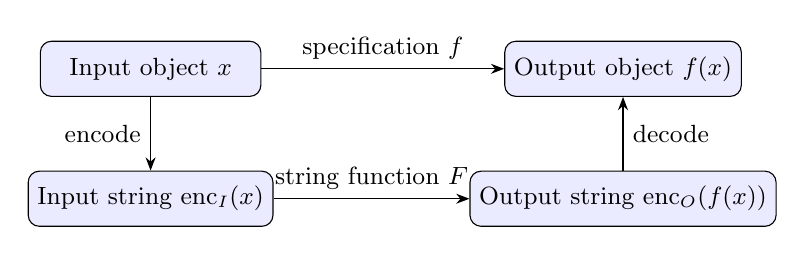
\begin{tikzpicture}[>=Stealth,
        box/.style={draw,rounded corners,fill=blue!8,align=center,
        minimum width=2.8cm,minimum height=0.7cm},
        every node/.style={font=\small}]
      \node[box] (x) at (0,0) {Input object $x$};
      \node[box] (y) at (6,0) {Output object $f(x)$};
      \node[box] (ex) at (0,-1.65) {Input string $\operatorname{enc}_I(x)$};
      \node[box] (ey) at (6,-1.65) {Output string $\operatorname{enc}_O(f(x))$};
      \draw[->] (x) -- node[above] {specification $f$} (y);
      \draw[->] (x) -- node[left] {encode} (ex);
      \draw[->] (ex) -- node[above] {string function $F$} (ey);
      \draw[->] (ey) -- node[right] {decode} (y);
    \end{tikzpicture}
  \end{center}
  \[
    F(\operatorname{enc}_I(x))=\operatorname{enc}_O(f(x)).
  \]
  \pause
  A Turing machine \textbf{computes} this transformation if, on each valid
  input encoding, it halts with the required output encoding in a designated
  tape region. Turing machines can produce outputs, not only accept/reject
  \cite{tm-functions}.
  \pause
  \par\smallskip
  This viewpoint covers tasks with finite, effectively representable data.
  It does \emph{not} assert that every specified $F$ is computable, or that
  arbitrary infinite objects have exact finite encodings.
\end{frame}

\begin{frame}{Why This Viewpoint Belongs in a CSE Curriculum}
  \small
  Lists, graphs, documents, and programs look different to an application,
  but their finite representations let us study them as string-processing tasks.
  \begin{block}{Three questions beyond implementing one algorithm}
    \begin{itemize}
      \item \textbf{Specification:} which input--output behavior is required?
        Correctness compares an implementation with that requirement.
      \pause
      \item \textbf{Computability:} can \emph{any} algorithm meet it on every
        valid input? Encoding a task does not answer this question.
      \pause
      \item \textbf{Complexity and models:} what resources are needed, and
        how does the chosen model affect the analysis?
    \end{itemize}
  \end{block}
  \pause
  \begin{exampleblock}{One sorting function, many implementations}
    Insertion sort and merge sort can implement the same mapping from lists
    to sorted lists. The specification stays fixed while the method and
    resource use change. ToC also asks what constraints apply to \emph{all}
    possible implementations, not only to these two.
  \end{exampleblock}
  Studying strings is therefore an abstraction of computational tasks,
  not a restriction of CSE to text editing.
\end{frame}

\begin{frame}{Decision Problems as Languages}
  \small
  A \textbf{decision problem} asks only for \texttt{YES} or \texttt{NO}.
  Encode its instances using a specified format. Its
  \textbf{language of yes-instances} is
  \[
    L=\{w\in\Sigma^*:w\text{ encodes an instance whose answer is yes}\}.
  \]
  Fix the encoding and how malformed inputs are handled (here, reject them).
  A general problem such as sorting produces an output object, not just
  a membership bit; decision languages capture its yes/no variants.
  Equivalently, a decider computes the characteristic function
  $\chi_L(w)=1$ when $w\in L$, and $\chi_L(w)=0$ otherwise.
  \pause
  \begin{exampleblock}{Examples}
    Binary strings with an odd number of $1$'s form one language.
    Encoded graphs having a path from a designated $s$ to $t$ form another.
    Asking for membership in these sets expresses the corresponding
    decision problems; the sets alone do not supply algorithms.
  \end{exampleblock}
  \pause
  \begin{block}{A relevant compiler connection}
    Lexing and parsing check aspects of a source program's form. A compiler
    also performs semantic checks and translates the program; its entire
    job is not just a syntax-membership test. Valid syntax does not by itself
    guarantee correct behavior.
  \end{block}
\end{frame}

% ==========================================
% Part 6: Grammars and Automata
% ==========================================
\section{Grammars and Automata}

\begin{frame}{Part 6: Grammars as Generators}
  \small
  A \textbf{grammar} specifies how to generate words. We preview a
  \emph{context-free grammar} (CFG); its full study comes in Slide Set~5.
  \pause
  \begin{block}{Grammar Quadruple}
    A CFG is a 4-tuple $G=(V,T,S,P)$:
    \begin{itemize}
        \item $V$: Finite set of \textbf{Variables} (Non-terminals).
        \item $T$: Finite set of \textbf{Terminals} (symbols from the alphabet). $V \cap T = \emptyset$.
        \item $S \in V$: The \textbf{Start Variable}.
        \item $P$: Finite set of \textbf{productions} $A\to\alpha$, where
          $A\in V$ and $\alpha\in(V\cup T)^*$.
    \end{itemize}
  \end{block}
  \pause
  If $A\to\alpha\in P$, one step replaces $uAv$ by $u\alpha v$:
  $uAv\Rightarrow u\alpha v$. The notation $\Rightarrow^*$ allows zero
  or more steps. A generated word contains only terminals:
  \[
    L(G)=\{w\in T^*:S\Rightarrow^*w\}.
  \]
  The rule arrow $\to$ and derivation arrow $\Rightarrow$ have different roles.
  More general grammars may replace longer left-hand sides; the one-variable
  restriction here is what makes the grammar context-free.
\end{frame}

\begin{frame}{A Grammar Example and Its Correctness}
  \small
  Use $V=\{S\}$, $T=\{a,b\}$ and productions $S\to aSb\mid\varepsilon$.
  The bar abbreviates two alternatives. A derivation is
  \[
    S\Rightarrow aSb\Rightarrow aaSbb\Rightarrow aabb.
  \]
  The intermediate $aaSbb$ is a \emph{sentential form}, not a terminal word.
  \pause
  \begin{block}{Claim: $L(G)=\{a^n b^n:n\ge0\}$}
    \textbf{Soundness.} After $k$ uses of $S\to aSb$, the form is $a^kSb^k$.
    Any terminating derivation then uses $S\to\varepsilon$, yielding $a^kb^k$.
    \par\smallskip
    \textbf{Completeness.} For any $n\ge0$, use the recursive rule exactly
    $n$ times and the empty rule once. This generates $a^nb^n$.
  \end{block}
  \pause
  The case $n=0$ gives $S\Rightarrow\varepsilon$.
  Examples suggest the pattern; the two inclusions prove it for every word.
  Without the terminating rule, this grammar would generate no terminal words.
\end{frame}

\begin{frame}{Automata as Recognizers}
  \small
  An \textbf{automaton} processes an input according to precise rules.
  Its model determines the available memory and allowed operations.
  
  \vspace{0.1cm}
  \begin{center}
  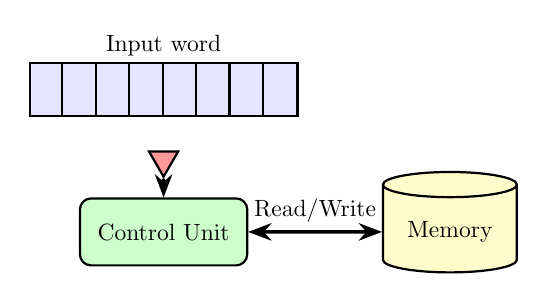
\begin{tikzpicture}[node distance=2.5cm, auto, thick,>=Stealth,scale=0.85,transform shape]
    % Input Tape
    \node[draw, rectangle, minimum width=4cm, minimum height=0.8cm, fill=blue!10] (input) {};
    \draw (input.south west) ++(0.5,0) -- ++(0,0.8);
    \draw (input.south west) ++(1.0,0) -- ++(0,0.8);
    \draw (input.south west) ++(1.5,0) -- ++(0,0.8);
    \draw (input.south west) ++(2.0,0) -- ++(0,0.8);
    \draw (input.south west) ++(2.5,0) -- ++(0,0.8);
    \draw (input.south west) ++(3.0,0) -- ++(0,0.8);
    \draw (input.south west) ++(3.5,0) -- ++(0,0.8);
    \node at ([yshift=0.65cm]input.center) {Input word};
    
    % Read Head
    \node[draw, regular polygon, regular polygon sides=3, shape border rotate=180, fill=red!40, minimum size=0.5cm, inner sep=0pt, below=0.5cm of input] (head) {};
    
    % Control Unit
    \node[draw, rectangle, rounded corners, minimum width=2.5cm, minimum height=1cm, fill=green!20, below=1.2cm of input] (control) {Control Unit};
    
    % Storage
    \node[draw, cylinder, shape border rotate=90, aspect=0.25, minimum width=2cm, minimum height=1.5cm, fill=yellow!20, right=2cm of control] (storage) {Memory};
    
    % Arrows
    \draw[->, very thick] (head) -- (control);
    \draw[<->, very thick] (control) -- (storage) node[midway, above] {Read/Write};
  \end{tikzpicture}
  \end{center}
  \vspace{0.2cm}
  \begin{itemize}
      \item \textbf{Finite automata:} finite-state memory only; no separate
        unbounded work storage.
      \item \textbf{Pushdown automata:} finite control plus a stack
        (last in, first out).
      \item \textbf{Turing machines:} finite control plus an unbounded
        read/write tape; the head moves locally, not by random access.
  \end{itemize}
  The diagram is schematic. In a standard one-tape Turing machine, the
  input is initially on the work tape itself.
\end{frame}

\begin{frame}{Several Models, Different Views of Computation}
  \small
  A \textbf{model of computation} fixes the machine's configurations,
  allowed steps, and input/output conventions. No single model serves
  every explanatory purpose.
  \begin{description}
    \item[Finite automata (DFA/NFA):] finite-state control; study what can
      be recognized with only finite memory.
    \item[Pushdown automata (PDA):] finite control plus a stack; model
      nested structure and stack-based recognition.
    \item[Turing machines (TM):] control plus an unbounded tape whose head
      moves locally; a simple general-purpose model for computability proofs.
  \end{description}
  \pause
  \begin{block}{Random Access Machine (RAM): the programming viewpoint}
    A program uses registers, addressed memory, arithmetic, and branches.
    ``Random access'' means access by address, not randomness. A word-RAM
    specifies word size and primitive-operation costs, making it useful for
    ordinary algorithm analysis~\cite{wordram}.
  \end{block}
  \pause
  RAM is a model \emph{alongside} TM, not the hidden basis of every ToC
  model. Standard effective RAM and TM models simulate each other;
  runtime comparisons require explicit cost assumptions~\cite{model-simulation}.
\end{frame}

\begin{frame}{Other Models You Will Encounter in CSE}
  \small
  \begin{description}
    \item[Lambda calculus:] computation by function abstraction, application,
      and substitution; a foundation for functional programming.
    \pause
    \item[Boolean circuits:] networks of logic gates transform input bits
      into output bits; connect computation to digital hardware.
      One fixed circuit has fixed input and output sizes; varying input
      lengths require a circuit family~\cite{circuit-model}.
    \pause
    \item[Cellular automata:] cells repeatedly update their states using
      local neighbors; model parallel, spatial computation. Some rule
      systems can simulate a Turing machine, but not every rule system can
      do so~\cite{other-models}.
  \end{description}
  \pause
  \begin{block}{Different presentations do not always mean different power}
    The untyped lambda calculus and standard general-purpose TM/RAM models
    describe the same computable functions, under effective encodings
    \cite{other-models}. Finite automata and one-stack PDAs are more restricted.
    A single fixed Boolean circuit is not a general-purpose machine for
    arbitrarily long inputs.
  \end{block}
  Model equivalence concerns what can be computed; it does not automatically
  equate time, memory, or implementation convenience.
\end{frame}

\begin{frame}{Recognizing Is Not Always Deciding}
  \small
  \begin{block}{Two different requirements for a language $L$}
    A \textbf{decider} halts on every input, accepting exactly the words
    in $L$ and rejecting all others.
    \par\smallskip
    A \textbf{recognizer} accepts every word in $L$. On a word outside $L$,
    it never accepts, but may reject or run forever.
  \end{block}
  \pause
  \begin{itemize}
    \item Every decider is a recognizer; a recognizer need not be a decider.
    \item A DFA always finishes after reading its finite input, so it decides
      its language. General Turing-machine recognizers may not halt.
    \item A grammar generates words; a machine tests input words. These
      are different descriptions, and equivalence requires a theorem.
  \end{itemize}
  \pause
  \textbf{Road ahead:} finite automata and regular grammars describe the
  same languages; pushdown automata and CFGs describe the same languages.
  Neither statement says that every language has such a description.
\end{frame}

% ==========================================
% Part 7: Proof Techniques
% ==========================================
\section{Proof Techniques}

\begin{frame}{Part 7: Choosing a Proof Method}
  \small
  \begin{itemize}
    \item \textbf{Direct proof of $P\Rightarrow Q$:} assume $P$ and derive $Q$.
    \item \textbf{Contrapositive:} instead prove $\neg Q\Rightarrow\neg P$.
    \item \textbf{Contradiction:} assume the claim is false and derive an
      impossibility. For $P\Rightarrow Q$, assume $P$ and $\neg Q$.
    \item \textbf{Equality of sets or languages:} prove both inclusions.
    \item \textbf{Induction:} establish a base case and a step that covers
      every larger case.
  \end{itemize}
  \pause
  \begin{exampleblock}{Contrapositive: if $n^2$ is even, then $n$ is even}
    If $n$ is odd, write $n=2k+1$ for some integer $k$. Then
    $n^2=4k^2+4k+1=2(2k^2+2k)+1$ is odd. This proves the contrapositive.
  \end{exampleblock}
  \pause
  State the claim and assumptions before calculating. A diagram or a few
  test inputs may guide a proof, but do not settle an infinite family of cases.
\end{frame}

\begin{frame}{Proof by Contradiction}
  \small
  In a proof by contradiction, we assume the statement is \textit{false}, and show that this assumption leads to a logical impossibility.
  \pause
  \begin{block}{Theorem: $\sqrt{2}$ is irrational}
    \textbf{Proof:} Assume for contradiction that $\sqrt{2}$ is rational. 
    \begin{enumerate}
        \item Write $\sqrt{2}=m/n$ with positive integers $m,n$ in lowest
          terms: $\gcd(m,n)=1$.
        \item Squaring both sides: $2 = \frac{m^2}{n^2} \implies 2n^2 = m^2$.
        \item By the parity fact just proved, $m$ is even. Write $m=2k$.
        \pause
        \item Substitute back: $2n^2 = (2k)^2 = 4k^2 \implies n^2 = 2k^2$.
        \item This means $n^2$ is even, so $n$ must be even.
        \item If $m$ and $n$ are both even, they share a common factor of 2. This contradicts our assumption! Therefore, $\sqrt{2}$ must be irrational. \hfill $\blacksquare$
    \end{enumerate}
  \end{block}
\end{frame}

\begin{frame}{Proof by Induction}
  \small
  To prove a property $P(n)$ holds for all integers $n \ge 0$:
  \begin{itemize}
      \item \textbf{Basis:} Prove $P(0)$ is true.
      \item \textbf{Inductive step:} for an arbitrary $k\ge0$, assume $P(k)$
        and prove $P(k+1)$. Do not assume $P(k+1)$ while proving it.
  \end{itemize}
  \pause
  \begin{block}{Theorem: a binary tree of height at most $n$ has at most $2^n$ leaves}
    Use height measured in edges and at most two children per node.
    \begin{itemize}
        \item \textbf{Base:} height at most $0$ means a single root, with
          one leaf, and $1=2^0$.
        \item \textbf{Hypothesis:} every binary tree of height at most $k$
          has at most $2^k$ leaves.
        \pause
        \item \textbf{Step:} a tree of height at most $k+1$ is either a
          single leaf or has one or two child subtrees, each of height at
          most $k$. Their leaves total at most $2\cdot2^k=2^{k+1}$.
          The single-leaf case also satisfies the bound.
    \end{itemize}
  \end{block}
  The phrase ``at most'' lets the hypothesis apply to unequal-height
  subtrees. Equality is attained when every internal node has two children
  and every leaf is at depth $n$.
\end{frame}

\begin{frame}{Structural Induction: A String Identity}
  \small
  Finite strings are built from $\varepsilon$ by repeatedly appending one
  symbol. Proving a base case and an append-symbol case is induction on length.
  \begin{block}{Example: $(xy)^R=y^Rx^R$ for all strings $x,y$}
    Fix an arbitrary $x$ and induct on $y$.
    \par\smallskip
    \textbf{Base:} $y=\varepsilon$ gives
    $(x\varepsilon)^R=x^R=\varepsilon^Rx^R$.
    \pause
    \par\smallskip
    \textbf{Step:} let $y=za$, where $a$ is one symbol, and assume
    $(xz)^R=z^Rx^R$. By the definition $(wa)^R=aw^R$,
    \[
      (xza)^R=a(xz)^R=az^Rx^R=(za)^Rx^R.
    \]
    Thus the claim holds for every $y$, and $x$ was arbitrary too.
  \end{block}
  \pause
  The same pattern proves properties of recursively built expressions or
  derivation trees: cover every base constructor and every recursive constructor.
\end{frame}

% ==========================================
% Pedagogical Enhancements (Exercises)
% ==========================================
\section{Exercises and Review}

\begin{frame}{Checkpoint Exercises 1: Sets, Relations, and Logic}
  \small
  \begin{enumerate}
      \item \textbf{Sets:} Let $A = \{1, 2, 3\}$ and $B = \{3, 4, 5\}$. 
      \newline What is $(A \cup B) - (A \cap B)$?
      \vspace{0.5cm}
      \item \textbf{Relations:} A relation $R$ on $\mathbb{Z}$ is defined as $x R y$ if $x \le y$. 
      \newline Which equivalence property does this relation \textit{fail}? (Reflexivity, Symmetry, or Transitivity?)
      \vspace{0.5cm}
      \item \textbf{Boolean Logic:} Evaluate the following expression, given $P = 1, Q = 0, R = 1$:
      \[ \neg P \vee Q \wedge R \]
  \end{enumerate}
\end{frame}

\begin{frame}{Checkpoint Exercises 2: Strings and Grammars}
  \small
  \begin{enumerate}
      \setcounter{enumi}{3}
      \item \textbf{Strings:} Let $\Sigma = \{0, 1\}$. How many strings are in $\Sigma^*$ of length exactly 3? List them.
      \vspace{0.5cm}
      \item \textbf{Grammars:} Consider the grammar $G$:
      \begin{align*}
          S &\rightarrow a A \\
          A &\rightarrow b S \mid \varepsilon
      \end{align*}
      Show the derivation sequence for the string $ababa$. What is the general language $L(G)$ described in English?
  \end{enumerate}
\end{frame}

\begin{frame}{Checkpoint Exercises 3: Proofs and Graphs}
  \small
  \begin{enumerate}
      \setcounter{enumi}{5}
      \item \textbf{Graphs:} A finite simple undirected graph has $v$ vertices
        and $e$ edges. The degree of a vertex is the number of incident
        edges. Prove directly that the sum of all vertex degrees is $2e$.
      \vspace{0.5cm}
      \item \textbf{Induction:} We want to prove by induction that $1 + 2 + \dots + n = \frac{n(n+1)}{2}$. 
      \newline State explicitly what the \textbf{Basis} and the \textbf{Inductive Hypothesis} are for this proof.
  \end{enumerate}
\end{frame}

\begin{frame}{Checkpoint Exercises 4: Boundaries and Quantifiers}
  \small
  \begin{enumerate}
    \setcounter{enumi}{7}
    \item Negate $\forall x\in D\;\exists y\in D\;R(x,y)$, showing both
      quantifiers. Explain why choosing a single $y$ in advance is not
      generally allowed in the original statement.
    \pause
    \item For $L=\{\varepsilon,a\}$, compute $L^2$, and decide whether
      $L^+=L^*\setminus\{\varepsilon\}$. Explain rather than just answer yes/no.
    \pause
    \item A rooted tree has a root with two children; the left child is a
      leaf and the right child has two leaf children. Find the tree's height,
      its number of leaves, and the depth and height of the left child.
  \end{enumerate}
  \begin{block}{Self-check before submitting a proof}
    Have you fixed the universe or alphabet? Included the empty case?
    Proved the stated direction? Used a hypothesis strong enough for
    every recursive subcase?
  \end{block}
\end{frame}

\begin{frame}{Summary and Bridge to Finite Automata}
  \small
  \begin{itemize}
    \item Sets ignore order; tuples and strings do not. A language is a set
      of finite strings, not a single string.
    \item Functions have specified domains and codomains. Equivalence
      relations partition a set into classes.
    \item Quantifier order determines what choices may depend on what;
      negation reverses universal and existential quantifiers.
    \item Graphs describe connections; rooted trees describe hierarchy.
      Depth and height count edges in different directions.
    \item Grammars generate words; recognizers accept words; deciders
      additionally halt on every input.
    \item A problem specifies correct outputs; an encoding represents its
      instances. Runtime depends on input length and the chosen machine model.
    \item Proofs need explicit assumptions, all required directions, and
      boundary cases---not just convincing examples.
  \end{itemize}
  \pause
  \begin{block}{Next: Slide Set 2}
    A finite automaton combines sets, functions, and a labeled directed graph.
    Its states remember input-prefix information; induction justifies this meaning.
  \end{block}
\end{frame}

\appendix
\section{Appendix: Worked Answers and Further Foundations}
\subsection{Checkpoint Solutions}

\begin{frame}{Solutions 1--3: Sets, Relations, and Logic}
  \small
  \begin{enumerate}
    \item $A\cup B=\{1,2,3,4,5\}$ and $A\cap B=\{3\}$, so
      $(A\cup B)\setminus(A\cap B)=\{1,2,4,5\}$.
      This operation is the \emph{symmetric difference}: membership in
      exactly one set.
    \pause
    \item The relation $x\le y$ on $\mathbb{Z}$ is reflexive and transitive,
      but not symmetric: $3\le4$ while $4\not\le3$. Thus it is not an
      equivalence relation. A relation may satisfy some properties without
      satisfying all of them.
    \pause
    \item For $P=1$, $Q=0$, $R=1$,
      \[
        \neg P\vee(Q\wedge R)=0\vee(0\wedge1)=0.
      \]
      The parentheses show the intended precedence explicitly.
  \end{enumerate}
\end{frame}

\begin{frame}{Solutions 4--5: Strings and a Grammar}
  \small
  \textbf{4.} There are $2^3=8$ length-three binary words:
  $000,001,010,011,100,101,110,111$.
  \pause
  \par\medskip
  \textbf{5.} For $S\to aA$, $A\to bS\mid\varepsilon$, a derivation is
  \[
    S\Rightarrow aA\Rightarrow abS\Rightarrow abaA
      \Rightarrow ababS\Rightarrow ababaA\Rightarrow ababa.
  \]
  \begin{block}{The full language, not just one example}
    $L(G)=\{(ab)^n a:n\ge0\}$: alternating $a$'s and $b$'s beginning
    and ending with $a$.
    \par\smallskip
    Each cycle $S\Rightarrow aA\Rightarrow abS$ adds one $ab$.
    Termination uses $S\Rightarrow aA\Rightarrow a$, so every terminal
    derivation has the stated form. Conversely, take $n$ cycles and then
    terminate to generate any $(ab)^na$.
  \end{block}
  \pause
  The shortest word is $a$, not $\varepsilon$. Only $A$ can derive $\varepsilon$ here;
  the start variable still forces an $a$ before termination.
\end{frame}

\begin{frame}{Solutions 6--7: Double Counting and Induction}
  \small
  \textbf{6. Handshaking argument.} Count vertex--edge incidences.
  Summing vertex degrees counts each incidence once. Each edge of a simple
  undirected graph has two distinct endpoints, so contributes two incidences.
  Hence $\sum_{v\in V}\deg(v)=2|E|$.
  \pause
  \begin{block}{7. Sum of the first $n$ positive integers, $n\ge1$}
    \textbf{Base:} $n=1$ gives $1=1(1+1)/2$.
    \par\smallskip
    \textbf{Hypothesis:} for an arbitrary $k\ge1$, assume
    $1+\cdots+k=k(k+1)/2$.
    \par\smallskip
    \textbf{Step:}
    \[
      1+\cdots+k+(k+1)
      =\frac{k(k+1)}2+(k+1)
      =\frac{(k+1)(k+2)}2.
    \]
    This is the formula for $k+1$, completing the induction.
  \end{block}
  Starting at $n=0$ also works if the empty sum is defined to be zero;
  make that convention explicit.
\end{frame}

\begin{frame}{Solutions 8--10: Boundary Cases Matter}
  \small
  \begin{enumerate}
    \setcounter{enumi}{7}
    \item The negation is $\exists x\in D\;\forall y\in D\;\neg R(x,y)$.
      In the original statement, a suitable $y$ may depend on $x$;
      requiring one common witness changes the assertion.
    \pause
    \item $L^2=\{\varepsilon,a,aa\}$. Duplicate ways to form $a$ do not
      produce duplicate set elements. Both $L^+$ and $L^*$ equal
      $\{a^n:n\ge0\}$, since an empty factor is allowed. Thus $L^+$
      contains $\varepsilon$, whereas $L^*\setminus\{\varepsilon\}$ does not.
    \pause
    \item The tree has height $2$ and three leaves. The left child has
      depth $1$ and height $0$. The leaf bound gives $3\le2^2=4$;
      it is an upper bound, not a formula for the exact number of leaves.
  \end{enumerate}
\end{frame}

\subsection{Computational Tasks as String Transformations}

\begin{frame}{One Function, Two Representations: Sorting}
  \small
  Return to the sorting problem. For a simple format, let list entries be
  single decimal digits. Encode a list using brackets and comma-separated
  digits; the empty list is \texttt{[]}.
  \begin{block}{Object-level specification}
    \[
      f((3,1,3,2))=(1,2,3,3).
    \]
    The output is nondecreasing and preserves every element's multiplicity.
  \end{block}
  \pause
  \begin{block}{The corresponding string function}
    \[
      F(\texttt{[3,1,3,2]})=\texttt{[1,2,3,3]},\qquad
      F(\texttt{[]})=\texttt{[]}.
    \]
    Decoding the output string gives exactly the required output list.
    This is the same task expressed at a different level, not a new problem.
  \end{block}
  \pause
  A RAM program may manipulate an array; a Turing machine may manipulate
  a tape representation. If both meet this specification on every valid
  list, they compute the same function despite different internal steps.
  Correctness concerns the input--output relationship, not identical execution.
\end{frame}

\begin{frame}{A Turing Machine Producing an Output: Increment}
  \small
  The numerical task is $f(n)=n+1$ for $n\in\mathbb{N}$.
  Use binary, with $0$ encoded as \texttt{0} and no leading zeros otherwise.
  The string task is $F(\operatorname{bin}(n))=\operatorname{bin}(n+1)$.
  \[
    13\mapsto14\qquad\text{becomes}\qquad
    \texttt{1101}\mapsto\texttt{1110}.
  \]
  \pause
  \begin{block}{A tape-level strategy, not yet a formal transition table}
    On a tape with blank cells on both sides of the input:
    \begin{enumerate}
      \item Scan right to the first blank, then move left to the last bit.
      \item Carry a $1$: replace each encountered $1$ by $0$ and move left.
      \item At a $0$, write $1$ and halt. If the carry reaches the blank
        before the word, write $1$ there and halt instead.
    \end{enumerate}
  \end{block}
  \pause
  For \texttt{1101}, the changed tape word goes
  $\texttt{1101}\to\texttt{1100}\to\texttt{1110}$.
  For \texttt{111}, the final output is \texttt{1000}.
  Read the final contiguous block of bits as the output.
  \par\smallskip
  The finite scan and carry always terminate on valid input. The machine
  has \emph{computed a value}, not merely answered a membership question.
\end{frame}

\begin{frame}{The Graph Example: A Bit Answer or a Structured Answer?}
  \small
  Reuse the main-slide instance: edges $1\to2\to3$, with $s=1,t=3$.
  Its input encoding is
  \[
    \texttt{11\#010001000\#1\#11}.
  \]
  The \emph{output specification} determines which function we want.
  \begin{block}{Reachability as a decision function}
    Output \texttt{1} if a path exists, and \texttt{0} otherwise.
    For this input, the output string is \texttt{1}.
    This is the language-membership viewpoint.
  \end{block}
  \pause
  \begin{block}{Route production as a string-output function}
    Specify the shortest path, breaking ties lexicographically by vertex
    sequence; return \texttt{NONE} if there is no path.
    Encode a path as its vertex numbers in binary, separated by \texttt{\#}.
    Here the answer $(1,2,3)$ becomes \texttt{1\#10\#11}.
  \end{block}
  \pause
  Both tasks process the \emph{same input representation}, but compute
  different outputs. The tie-breaking rule makes the second answer unique.
  Without it, ``return any route'' specifies allowed input--output pairs
  rather than a unique function.
\end{frame}

\begin{frame}{Programs Are Data Too: The Interpreter Perspective}
  \small
  A program has a finite description, so it too can be encoded as a string.
  An interpreter takes \emph{two pieces of data}: a program description and
  that program's input, packaged in an unambiguous pair encoding.
  \[
    \langle P,x\rangle
      \quad\xrightarrow{\text{interpreter or universal machine}}\quad
      \langle y\rangle
      \qquad\text{if }P(x)\text{ halts with }y.
  \]
  \pause
  \begin{exampleblock}{A connection to everyday programming}
    Let $P$ be a program for incrementing a natural number, and let $x=13$.
    The interpreter receives their encodings and eventually produces the
    encoding of $14$. Changing $P$ changes the transformation without
    changing the interpreter itself.
  \end{exampleblock}
  \pause
  \begin{block}{Why termination now matters}
    If $P(x)$ runs forever, a faithful interpreter may do so too.
    Its behavior is a \emph{partial} string function: some inputs have no
    returned output. A universal Turing machine formalizes this idea
    \cite{universal-machine}.
  \end{block}
  This connects strings, programs, simulation between models, and the
  question of which computational tasks can be solved at all.
\end{frame}

\subsection{References}

\begin{frame}{Further Reading: Problems, Encodings, and RAM Models}
  \small
  \setbeamertemplate{bibliography item}[text]
  \begin{thebibliography}{9}
    \bibitem[DKS20]{algorithms-intro}
      Erik Demaine, Jason Ku, and Justin Solomon,
      \href{https://ocw.mit.edu/courses/6-006-introduction-to-algorithms-spring-2020/477c78e0af2df61fa205bcc6cb613ceb_MIT6_006S20_lec1.pdf}
      {MIT 6.006, Lecture 1: Introduction}, Spring 2020.
      Input--output problem specifications, algorithms, and word-RAM costs.
    \bibitem[M]{wordram}
      Pat Morin, \emph{Open Data Structures},
      \href{https://opendatastructures.org/ods-cpp/1_4_Model_Computation.html}
      {Section 1.4: The Model of Computation}.
      Word size, addressable memory, and primitive operations.
    \bibitem[B]{model-simulation}
      Boaz Barak, \emph{Introduction to Theoretical Computer Science},
      \href{https://introtcs.org/public/lec_11_running_time.html}
      {Modeling Running Time}.
      Formal RAM/Turing-machine simulations and their cost assumptions.
  \end{thebibliography}
  The list and graph formats illustrate input--output representations;
  they are teaching examples, not universal serialization standards.
\end{frame}

\begin{frame}{Further Reading: Functions and Alternative Models}
  \footnotesize
  \setbeamertemplate{bibliography item}[text]
  \begin{thebibliography}{9}
    \bibitem[C19]{tm-functions}
      Cornell CS 4820, 2019,
      \href{https://www.cs.cornell.edu/courses/cs4820/2019sp/handouts/computability.pdf}
      {\emph{Limits of Computability}}. Turing machines computing partial
      functions from input strings to output strings.
    \bibitem[BC]{circuit-model}
      Boaz Barak, \emph{Introduction to Theoretical Computer Science},
      \href{https://introtcs.org/public/lec_03_computation.html}
      {Defining Computation}. Functions as specifications and circuits
      as implementations for fixed input/output sizes.
    \bibitem[BM]{other-models}
      Boaz Barak, same text,
      \href{https://introtcs.org/public/lec_07_other_models.html}
      {Equivalent Models of Computation}. Lambda calculus, cellular
      automata, and simulation between models.
    \bibitem[C17]{universal-machine}
      Cornell CS 2800, Spring 2017,
      \href{https://www.cs.cornell.edu/courses/cs2800/2017sp/lectures/lec28-turing.html}
      {Turing Machines}. Encoding machines and universal simulation.
  \end{thebibliography}
  The purpose here is to connect computational specifications to CSE
  practice; formal machine definitions and equivalence proofs come later.
\end{frame}

\begin{frame}{References and Suggested Teaching Use}
  \small
  \setbeamertemplate{bibliography item}[text]
  \begin{thebibliography}{9}
    \bibitem[S13]{sipser}
      Michael Sipser, \emph{Introduction to the Theory of Computation},
      3rd ed., Cengage, 2013. Chapter~0: mathematical notions,
      definitions, theorems, and proofs.
    \bibitem[LR23]{linz}
      Peter Linz and Susan H. Rodger,
      \emph{An Introduction to Formal Languages and Automata}, 7th ed.,
      Jones \& Bartlett Learning, 2023. Introductory mathematical
      preliminaries, languages, grammars, and automata.
    \bibitem[LLM15]{mcs}
      Eric Lehman, F. Thomson Leighton, and Albert R. Meyer,
      \href{https://ocw.mit.edu/courses/6-042j-mathematics-for-computer-science-spring-2015/mit6_042js15_textbook.pdf}
      {\emph{Mathematics for Computer Science}}, MIT, 2015.
      Supplementary practice in logic, proof methods, relations, and graphs.
  \end{thebibliography}
  Use the main sequence as a prerequisite review and the appendix for
  worked answers and deeper encoding/model examples. These exercises
  are course practice, not claimed to be numbered textbook problems.
\end{frame}

\end{document}
